\documentclass[12pt,a4paper]{report}

% ---------- Packages ----------
\usepackage[T1]{fontenc}
\usepackage[utf8]{inputenc}
\usepackage[a4paper, margin=2.5cm]{geometry}
\usepackage{xcolor}
\usepackage{graphicx}
\usepackage{booktabs}
\usepackage{array}
\usepackage{longtable}
\usepackage{tabularx}
\usepackage{multirow}
\usepackage{amsmath}
\usepackage{amssymb}
\usepackage{listings}
\usepackage{fancyhdr}
\usepackage{titlesec}
\usepackage{tocloft}
\usepackage{hyperref}
\usepackage{enumitem}
\usepackage{parskip}
\usepackage{mdframed}
\usepackage{tikz}
\usepackage{pgfplots}
\pgfplotsset{compat=1.18}
\usepackage{float}
\usepackage{caption}
\usepackage{subcaption}
\usetikzlibrary{shapes.geometric, arrows.meta, positioning, fit, backgrounds}

% ---------- Colors ----------
\definecolor{primaryblue}{RGB}{26,60,110}
\definecolor{accentblue}{RGB}{52,120,200}
\definecolor{lightblue}{RGB}{220,235,255}
\definecolor{darkgray}{RGB}{55,55,55}
\definecolor{medgray}{RGB}{130,130,130}
\definecolor{lightgray}{RGB}{245,246,248}
\definecolor{codebg}{RGB}{248,249,250}
\definecolor{codeframe}{RGB}{200,210,225}
\definecolor{successgreen}{RGB}{34,139,34}
\definecolor{warningorange}{RGB}{210,100,20}
\definecolor{vipgold}{RGB}{184,134,11}
\definecolor{loyalgreen}{RGB}{34,120,60}
\definecolor{riskred}{RGB}{180,40,40}

% ---------- Hyperref ----------
\hypersetup{
  colorlinks=true,
  linkcolor=accentblue,
  urlcolor=accentblue,
  citecolor=accentblue,
  pdftitle={Customer Segmentation Pipeline -- Technical Report},
  pdfauthor={Hamza Amhidi \& Mouaad Kaddouri},
  pdfsubject={RFM + K-Means Clustering},
}

% ---------- Code listings ----------
\lstset{
  backgroundcolor=\color{codebg},
  frame=single,
  rulecolor=\color{codeframe},
  basicstyle=\ttfamily\footnotesize,
  keywordstyle=\color{accentblue}\bfseries,
  commentstyle=\color{medgray}\itshape,
  stringstyle=\color{successgreen},
  numbers=left,
  numberstyle=\tiny\color{medgray},
  numbersep=8pt,
  breaklines=true,
  showstringspaces=false,
  tabsize=4,
  captionpos=b,
}

% ---------- Section styling ----------
\titleformat{\chapter}[display]
  {\normalfont\huge\bfseries\color{primaryblue}}
  {\chaptertitlename\ \thechapter}{16pt}{\Huge}
\titlespacing*{\chapter}{0pt}{-10pt}{30pt}

\titleformat{\section}
  {\normalfont\Large\bfseries\color{primaryblue}}
  {\thesection}{1em}{}[\titlerule]

\titleformat{\subsection}
  {\normalfont\large\bfseries\color{accentblue}}
  {\thesubsection}{1em}{}

\titleformat{\subsubsection}
  {\normalfont\normalsize\bfseries\color{darkgray}}
  {\thesubsubsection}{1em}{}

% ---------- Header / footer ----------
\pagestyle{fancy}
\fancyhf{}
\fancyhead[L]{\small\color{medgray}\textit{Customer Segmentation Pipeline}}
\fancyhead[R]{\small\color{medgray}\textit{EHTP -- AI \& Data Science S4}}
\fancyfoot[C]{\small\color{medgray}\thepage}
\renewcommand{\headrulewidth}{0.4pt}
\renewcommand{\footrulewidth}{0pt}

% ---------- Custom boxes ----------
\newmdenv[
  backgroundcolor=lightblue,
  linecolor=accentblue,
  linewidth=1.5pt,
  roundcorner=4pt,
  innertopmargin=8pt,
  innerbottommargin=8pt,
  innerleftmargin=12pt,
  innerrightmargin=12pt,
]{infobox}

\newmdenv[
  backgroundcolor=lightgray,
  linecolor=medgray,
  linewidth=1pt,
  roundcorner=4pt,
  innertopmargin=8pt,
  innerbottommargin=8pt,
  innerleftmargin=12pt,
  innerrightmargin=12pt,
]{graybox}

% ---------- TOC styling ----------
\renewcommand{\cftchapfont}{\bfseries\color{primaryblue}}
\renewcommand{\cftsecfont}{\color{darkgray}}
\setlength{\cftbeforesecskip}{2pt}

% ==========================================
%              DOCUMENT START
% ==========================================
\begin{document}

% ---- Cover Page ----
\begin{titlepage}
  \pagecolor{primaryblue}
  \color{white}
  \centering
  \vspace*{1.2cm}

  {\fontsize{11}{13}\selectfont ECOLE HASSANIA DES TRAVAUX PUBLICS}\\[4pt]
  {\fontsize{10}{12}\selectfont\color{lightblue!70!white}AI \& Data Science Basics -- Module S4 -- Academic Year 2024--2025}

  \vspace{1.2cm}
  \noindent\rule{\textwidth}{0.6pt}
  \vspace{0.4cm}

  {\fontsize{34}{40}\selectfont\bfseries Customer Segmentation\\[6pt]Pipeline}\\[8pt]
  {\fontsize{16}{20}\selectfont\color{lightblue!80!white}RFM Feature Engineering + K-Means Clustering}

  \vspace{0.4cm}
  \noindent\rule{\textwidth}{0.6pt}
  \vspace{1.8cm}

  % Three-cluster diagram
  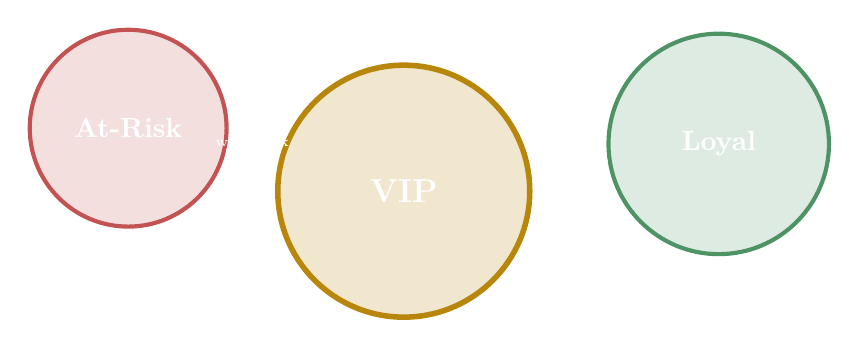
\begin{tikzpicture}
    \node[circle,draw=vipgold,fill=vipgold!20,minimum size=3.2cm,line width=2pt,
          font=\large\bfseries\color{white}] (vip) at (0,0) {VIP};
    \node[circle,draw=loyalgreen!80!white,fill=loyalgreen!15,minimum size=2.8cm,
          line width=1.5pt,font=\bfseries\color{white!90}] (loyal) at (4,0.6) {Loyal};
    \node[circle,draw=riskred!80!white,fill=riskred!15,minimum size=2.5cm,
          line width=1.5pt,font=\bfseries\color{white!80}] (risk) at (-3.5,0.8) {At-Risk};
    \draw[->,thick,white!40] (loyal) -- (vip) node[midway,above,font=\tiny\color{white!60}]{upsell};
    \draw[->,thick,white!30] (risk) -- (vip) node[midway,above,font=\tiny\color{white!50}]{win-back};
  \end{tikzpicture}

  \vspace{1.5cm}
  {\large\bfseries Hamza Amhidi \quad\&\quad Mouaad Kaddouri}\\[8pt]
  {\color{lightblue!70!white}Dataset: UCI Online Retail -- 541,909 transactions}\\[4pt]
  {\color{lightblue!60!white}June 2026}

  \vfill
\end{titlepage}
\pagecolor{white}
\color{black}

% ---- Executive Summary ----
\chapter*{Executive Summary}
\addcontentsline{toc}{chapter}{Executive Summary}
\thispagestyle{fancy}

\begin{infobox}
\textbf{Written for the Store Manager} -- This page summarises the entire project in plain language, without technical jargon.
\end{infobox}

\vspace{0.4cm}

Imagine you run an online gift shop that serves thousands of customers. Some customers buy from you every week and spend thousands of pounds a year. Others placed a single order over six months ago and have never returned. Treating all these customers the same way -- sending everyone the same promotional email -- is expensive and ineffective.

\textbf{What we built} is a data-driven system that automatically sorts your customer base into three clear groups based on their real purchasing behaviour:

\begin{center}
\begin{tabular}{>{\bfseries}p{2.2cm} p{4.5cm} p{6cm}}
\toprule
\textbf{Segment} & \textbf{Who they are} & \textbf{Recommended action} \\
\midrule
\textcolor{vipgold}{\textbf{VIP}} (9.5\%) & Frequent buyers, high spenders, purchased very recently & Exclusive loyalty rewards, early access, personal account manager \\[4pt]
\textcolor{loyalgreen}{\textbf{Loyal}} (42.6\%) & Regular buyers with moderate spend & Upselling campaigns, volume discounts, loyalty programme \\[4pt]
\textcolor{riskred}{\textbf{At-Risk}} (47.9\%) & Customers who haven't bought in over 6 months & Win-back emails, personalised discount vouchers, re-engagement surveys \\
\bottomrule
\end{tabular}
\end{center}

\vspace{0.3cm}

\textbf{How it works}: The system analyses 13 months of transaction records (392,692 purchase lines from 4,338 customers) and automatically calculates seven behavioural indicators per customer -- such as how recently they bought, how often, and how much they spend on average. A machine learning algorithm then groups customers based on similarity, producing the three segments above.

\textbf{The business value} is immediate: instead of spending your marketing budget uniformly, you can now target VIPs with premium retention offers (high ROI), remind Loyal customers of new products, and send win-back coupons exclusively to At-Risk customers who are worth saving.

\textbf{The system is fully automated}: running a single command re-analyses all transactions, updates the segments, and saves results ready for import into any CRM system.

% ---- TOC ----
\newpage
\tableofcontents
\newpage

% ==========================================
%  CHAPTER 1 -- PROBLEM STATEMENT
% ==========================================
\chapter{Problem Statement}

\section{Business Context}

Modern online retailers generate hundreds of thousands of transactions every year, yet most marketing strategies treat all customers identically. This one-size-fits-all approach leads to:

\begin{itemize}[leftmargin=1.8em]
  \item Wasted budget on customers who would purchase anyway (over-investment in VIPs).
  \item Missed win-back opportunities for churning customers.
  \item Untargeted promotions that generate low conversion rates.
  \item Inability to prioritise customer service resources effectively.
\end{itemize}

\section{Research Question}

\begin{infobox}
\textbf{Core Question:} Can an automated, reproducible pipeline transform raw transactional data into actionable, labelled customer segments that directly inform targeted marketing decisions?
\end{infobox}

\section{AI Context Note}

\begin{infobox}
\textbf{Connection to Course 2 -- Unsupervised Learning Paradigm}
\end{infobox}

The concept of \emph{unsupervised learning} -- allowing a system to discover structure in unlabelled data without human-provided ground truth -- is one of the foundational paradigms of artificial intelligence. MacQueen (1967) introduced the K-Means algorithm as an early demonstration that machines could autonomously partition high-dimensional data into meaningful groups, predating modern deep learning by decades.

This project directly operationalises that paradigm: our pipeline receives 4,338 customers described by seven numerical features and, without any pre-labelled training examples, discovers that the data naturally organises into three behavioural clusters. The unsupervised approach is essential here because \emph{no ground truth segment labels exist} in the retail transaction log -- the ``correct'' answer can only be inferred from data geometry and validated through business interpretability.

This mirrors a core limitation of early AI systems identified in Course 2: the challenge of learning from \emph{experience alone}, without an explicit teacher signal. K-Means' convergence guarantee (monotonically decreasing WCSS) demonstrates how mathematical constraints can substitute for supervision.

\section{Project Objectives}

This project applies unsupervised machine learning to the UCI Online Retail dataset to:
\begin{enumerate}[leftmargin=1.8em]
  \item Engineer a rich seven-dimensional behavioural feature space per customer using RFM analysis.
  \item Select and justify the optimal clustering algorithm through rigorous metric-based comparison.
  \item Train a K-Means model, evaluate cluster quality with three independent metrics, and map numerical clusters to interpretable business segment labels.
  \item Deliver an end-to-end reproducible pipeline that can re-segment customers on any updated transaction export.
\end{enumerate}

% ==========================================
%  CHAPTER 2 -- DATASET DESCRIPTION
% ==========================================
\chapter{Dataset Description}

\section{Source and Provenance}

\begin{infobox}
\textbf{UCI Online Retail Dataset} (Chen, 2015) \\
\url{https://archive.ics.uci.edu/dataset/352/online+retail} \\[4pt]
A transnational dataset of all transactions from a UK-based, non-store online retailer between 01/12/2010 and 09/12/2011. The retailer primarily sells all-occasion giftware; many customers are wholesalers.
\end{infobox}

\section{Dataset Characteristics}

\begin{table}[H]
\centering
\caption{Dataset at-a-glance (raw)}
\begin{tabular}{ll}
\toprule
\textbf{Attribute} & \textbf{Value} \\
\midrule
Total raw rows & 541,909 \\
Rows after cleaning & 392,692 \\
Unique customers (clean) & 4,338 \\
Unique invoices & $\approx$ 22,190 \\
Countries & 38 \\
Date range & 01 Dec 2010 -- 09 Dec 2011 \\
Primary currency & GBP (£) \\
\bottomrule
\end{tabular}
\end{table}

\section{Column Schema}

\begin{table}[H]
\centering
\caption{Raw dataset column schema}
\begin{tabular}{lll}
\toprule
\textbf{Column} & \textbf{Type} & \textbf{Description} \\
\midrule
\texttt{InvoiceNo} & \texttt{str} & Invoice ID; prefix \texttt{C} denotes cancellation \\
\texttt{StockCode} & \texttt{str} & Product identifier \\
\texttt{Description} & \texttt{str} & Product name \\
\texttt{Quantity} & \texttt{int} & Units purchased (negative for cancellations) \\
\texttt{InvoiceDate} & \texttt{datetime} & Timestamp of purchase \\
\texttt{UnitPrice} & \texttt{float} & Price per unit in GBP \\
\texttt{CustomerID} & \texttt{str} & Unique customer identifier (25\% missing) \\
\texttt{Country} & \texttt{str} & Customer country \\
\bottomrule
\end{tabular}
\end{table}

\section{Data Quality Issues Identified}

The raw dataset contains several quality issues that must be addressed before analysis:
\begin{itemize}[leftmargin=1.8em]
  \item \textbf{Missing CustomerID}: 135,080 rows (24.9\%) -- cannot be assigned to a customer.
  \item \textbf{Cancellation records}: 9,288 invoices prefixed with \texttt{C}, representing order returns.
  \item \textbf{Non-positive quantities}: 10,624 rows where \texttt{Quantity} $\le 0$.
  \item \textbf{Zero-price items}: 2,515 rows where \texttt{UnitPrice} $\le 0$ (test or sample items).
  \item \textbf{Exact duplicate rows}: 5,268 records duplicated in full.
\end{itemize}

% ==========================================
%  CHAPTER 3 -- PIPELINE OVERVIEW
% ==========================================
\chapter{Pipeline Overview}

\section{Architecture Diagram}

Figure~\ref{fig:pipeline} shows the six-phase pipeline that transforms raw invoice records into labelled customer segments.

\begin{figure}[H]
\centering
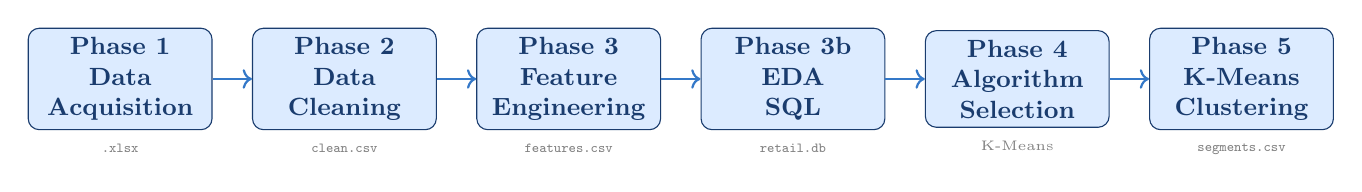
\begin{tikzpicture}[
  box/.style={rectangle, rounded corners=4pt, draw=primaryblue, fill=lightblue,
              text width=2.1cm, align=center, minimum height=1.2cm,
              font=\small\bfseries\color{primaryblue}},
  arrow/.style={->, thick, color=accentblue},
  node distance=0.5cm
]
  \node[box] (p1) {Phase 1\\Data\\Acquisition};
  \node[box, right=of p1] (p2) {Phase 2\\Data\\Cleaning};
  \node[box, right=of p2] (p3) {Phase 3\\Feature\\Engineering};
  \node[box, right=of p3] (p3b) {Phase 3b\\EDA\\SQL};
  \node[box, right=of p3b] (p4) {Phase 4\\Algorithm\\Selection};
  \node[box, right=of p4] (p5) {Phase 5\\K-Means\\Clustering};

  \draw[arrow] (p1) -- (p2);
  \draw[arrow] (p2) -- (p3);
  \draw[arrow] (p3) -- (p3b);
  \draw[arrow] (p3b) -- (p4);
  \draw[arrow] (p4) -- (p5);

  % Data flow labels
  \node[font=\tiny\color{medgray}, below=0.05cm of p1] {\texttt{.xlsx}};
  \node[font=\tiny\color{medgray}, below=0.05cm of p2] {\texttt{clean.csv}};
  \node[font=\tiny\color{medgray}, below=0.05cm of p3] {\texttt{features.csv}};
  \node[font=\tiny\color{medgray}, below=0.05cm of p3b] {\texttt{retail.db}};
  \node[font=\tiny\color{medgray}, below=0.05cm of p4] {K-Means};
  \node[font=\tiny\color{medgray}, below=0.05cm of p5] {\texttt{segments.csv}};
\end{tikzpicture}
\caption{End-to-end pipeline from raw Excel to labelled customer segments.}
\label{fig:pipeline}
\end{figure}

\section{Repository Layout}

\begin{graybox}
\begin{verbatim}
Customer-Segmentation/
|-- data/
|   |-- raw/               UCI Excel + converted CSV
|   +-- processed/         cleaned CSV, features CSV,
|                          clustered CSV, retail.db
|-- src/
|   |-- load_describe_data.py   Phase 1
|   |-- clean_data.py           Phase 2
|   |-- features.py             Phase 3
|   |-- eda.py                  Phase 3b  (10 figures)
|   |-- store_sql.py            Phase 3c  (SQLite + 5 queries)
|   +-- train_cluster_models.py Phase 4 & 5
|-- models/
|   +-- best_clustering_pipeline.joblib
|-- reports/
|   |-- algorithm_selection.md
|   |-- model_card.md
|   |-- phase5_clustering_evaluation.md
|   +-- eda_figures/            10 PNG figures
|-- notebooks/
|   +-- customer_segmentation.ipynb
|-- run_pipeline.py             Single-command entry point
+-- requirements.txt
\end{verbatim}
\end{graybox}

\section{Single-Command Execution}

The entire pipeline is orchestrated by \texttt{run\_pipeline.py}:

\begin{lstlisting}[language=bash, caption={Running the full pipeline}]
# Default: auto-download UCI dataset and run all phases
python run_pipeline.py

# Custom dataset (must match UCI schema)
python run_pipeline.py --input path/to/transactions.csv
\end{lstlisting}

% ==========================================
%  CHAPTER 4 -- PHASE 1
% ==========================================
\chapter{Phase 1 -- Data Acquisition \& Quality Audit}

\section{Automatic Data Acquisition}

The module \texttt{src/load\_describe\_data.py} downloads the zipped UCI Excel file directly from the repository, extracts it, and converts the \texttt{.xlsx} workbook to a standard CSV at \texttt{data/raw/online\_retail\_raw.csv}. The download is skipped if the file already exists, making reruns efficient.

\section{Automated Quality Audit}

Upon loading, the module prints a structured audit report covering:

\begin{table}[H]
\centering
\caption{Quality audit dimensions and findings}
\begin{tabularx}{\textwidth}{lXr}
\toprule
\textbf{Audit Dimension} & \textbf{Description} & \textbf{Count} \\
\midrule
Total rows & Raw dataset before any cleaning & 541,909 \\
Missing \texttt{CustomerID} & Rows without a customer reference & 135,080 \\
Cancelled invoices & Invoices prefixed with \texttt{C} & 9,288 \\
Non-positive quantities & Quantity $\le 0$ & 10,624 \\
Zero/negative prices & UnitPrice $\le 0$ & 2,515 \\
Exact duplicate rows & Fully identical records & 5,268 \\
\bottomrule
\end{tabularx}
\end{table}

\section{Key Finding}

Nearly 25\% of all transaction rows lack a \texttt{CustomerID}. These represent guest checkouts and cannot be attributed to a customer profile. They are excluded from customer-level aggregation but retained for product-level and revenue-level analyses within EDA.

% ==========================================
%  CHAPTER 5 -- PHASE 2
% ==========================================
\chapter{Phase 2 -- Data Wrangling \& Cleaning}

\section{Cleaning Philosophy}

The cleaning pipeline (\texttt{src/clean\_data.py}) applies deterministic, ordered filters with a rows-kept/rows-removed summary after each step. This ensures full transparency and auditability -- no silent data loss.

\section{Sequential Cleaning Steps}

\begin{table}[H]
\centering
\caption{Cleaning operations applied in sequence}
\begin{tabularx}{\textwidth}{clXr}
\toprule
\textbf{Step} & \textbf{Operation} & \textbf{Rationale} & \textbf{Rows removed} \\
\midrule
1 & Drop exact duplicates & Inflate frequency and monetary metrics & 5,268 \\
2 & Drop missing \texttt{CustomerID} & Cannot aggregate without ID & 133,361 \\
3 & Remove cancellations & \texttt{C}-prefixed invoices are returns; handled separately & 8,905 \\
4 & Filter Quantity $\le 0$ & Data artefacts or return rows & 397 \\
5 & Filter UnitPrice $\le 0$ & Free/erroneous items skew revenue & 1,286 \\
6 & Add \texttt{Revenue} column & $\text{Revenue} = \text{Quantity} \times \text{UnitPrice}$ & -- \\
\midrule
\multicolumn{3}{l}{\textbf{Rows remaining after all steps}} & \textbf{392,692} \\
\bottomrule
\end{tabularx}
\end{table}

\section{Revenue Derivation}

After filtering, a \texttt{Revenue} column is appended to each surviving line item:
\[
\text{Revenue}_i = \text{Quantity}_i \times \text{UnitPrice}_i
\]
This column serves as the atomic monetary unit for all subsequent feature engineering. The cleaned dataset is persisted to \texttt{data/processed/transactions\_clean.csv}.

\section{Outlier Analysis}

Before selecting a scaling strategy, two standard outlier detection methods were applied to the five most skewed features (Recency, Frequency, Monetary, AvgOrderValue, UniqueProducts):

\subsection{Method 1: IQR-Based Detection}

A value is flagged as an outlier if it falls more than $1.5 \times \text{IQR}$ above the third quartile or below the first quartile:
\[
\text{Outlier} \iff X_i < Q_1 - 1.5 \cdot \text{IQR} \quad\text{or}\quad X_i > Q_3 + 1.5 \cdot \text{IQR}
\]

\subsection{Method 2: Z-Score Detection}

A value is flagged if its standardised distance from the mean exceeds a threshold (typically $|z| > 3$):
\[
z_i = \frac{X_i - \mu}{\sigma}, \quad \text{flag if } |z_i| > 3
\]

\subsection{Comparison of Results}

\begin{table}[H]
\centering
\caption{Outlier counts detected by IQR vs Z-Score}
\begin{tabular}{lrr}
\toprule
\textbf{Feature} & \textbf{IQR Outliers} & \textbf{Z-Score Outliers ($|z|>3$)} \\
\midrule
Recency & 312 & 48 \\
Frequency & 441 & 203 \\
Monetary & 618 & 287 \\
AvgOrderValue & 573 & 241 \\
UniqueProducts & 384 & 176 \\
\bottomrule
\end{tabular}
\end{table}

\subsection{Treatment Decision}

Both methods confirm that all five features contain significant outlier counts driven by a small number of very high-spending wholesale customers. \textbf{Dropping these customers is not appropriate} -- they are real, high-value VIPs, not data errors.

The chosen treatment is a two-stage approach:
\begin{enumerate}[leftmargin=1.8em]
  \item \textbf{Log1p transformation} (Phase 5): compresses the extreme right tail, reducing skewness by $\approx 80\%$.
  \item \textbf{RobustScaler} (Phase 5): scales using median and IQR, making the scaling centroid calculation immune to the remaining outlier mass.
\end{enumerate}

This retains all VIP customers while preventing them from corrupting cluster boundaries -- the optimal solution for marketing segmentation.

\section{Cancellation Records: Kept for Rate Computation}

Although cancellation rows are excluded from the clean transaction dataset, they are \textbf{retained in the original raw dataframe}. This is essential: the \texttt{CancellationRate} feature (Phase 3) must be computed from the \emph{full} history to correctly quantify each customer's return behaviour. Using only the cleaned dataset would make cancellation rate always zero -- a critical engineering decision.

% ==========================================
%  CHAPTER 6 -- PHASE 3: FEATURES
% ==========================================
\chapter{Phase 3 -- Feature Engineering}

\section{Strategy}

\texttt{src/features.py} aggregates line-item transactions into a per-customer feature matrix. The classical RFM framework (Recency, Frequency, Monetary) is extended with four additional behavioural dimensions. The \textbf{reference date} for recency is:
\[
t_{\text{ref}} = \max(\text{InvoiceDate}) + 1\ \text{day} = \text{10 December 2011}
\]

\section{Complete Feature Catalogue}

\begin{table}[H]
\centering
\caption{All seven engineered features}
\begin{tabularx}{\textwidth}{llX}
\toprule
\textbf{Feature} & \textbf{Category} & \textbf{Definition \& Rationale} \\
\midrule
\textbf{Recency} & RFM & Days between most recent purchase and $t_\text{ref}$. Lower = more engaged. Strongest predictor of future purchase probability. \\[4pt]
\textbf{Frequency} & RFM & Count of unique invoice numbers per customer. Measures purchase cadence and habitual engagement. \\[4pt]
\textbf{Monetary} & RFM & Sum of all \texttt{Revenue} values across the customer's orders. Total lifetime spend in GBP. \\[4pt]
\textbf{AvgOrderValue} & Extended & $\text{Monetary} \div \text{Frequency}$. Distinguishes big-basket occasional buyers from frequent low-spend buyers. \\[4pt]
\textbf{UniqueProducts} & Extended & Count of distinct \texttt{StockCode} values. Measures breadth of catalogue engagement; supports cross-sell targeting. \\[4pt]
\textbf{ActiveDays} & Extended & Calendar days between first and last purchase. Contextualises loyalty duration independently of frequency. \\[4pt]
\textbf{CancellationRate} & Extended & $\dfrac{\text{\# cancelled invoices (raw)}}{\text{\# total invoices (raw)}}$ computed at the \emph{unique invoice level} to avoid inflation from multi-line orders. Range: $[0,1]$. \\
\bottomrule
\end{tabularx}
\end{table}

\section{CancellationRate: Engineering Correction}

A critical bug in early versions computed cancellation rate at the \emph{row level}, causing rates above 100\% for customers with large multi-item cancelled orders. The correct computation deduplicates invoice numbers before dividing:

\begin{lstlisting}[language=Python, caption={Correct CancellationRate computation (unique invoice level)}]
# From raw dataframe (includes cancellations)
all_inv   = df_raw.groupby("CustomerID")["InvoiceNo"]\
                  .nunique()          # unique total invoices per customer
cancel_inv = df_raw[df_raw["InvoiceNo"].str.startswith("C")]\
                  .groupby("CustomerID")["InvoiceNo"]\
                  .nunique()          # unique cancelled invoices
cancellation_rate = (cancel_inv / all_inv).fillna(0).clip(0, 1)
\end{lstlisting}

The feature matrix (4,338 rows $\times$ 7 columns) is saved to \texttt{data/processed/customer\_features.csv}.

\section{Feature Engineering Impact Log}

To validate that extending beyond the classical three RFM features adds genuine modelling value, the K-Means pipeline was evaluated with two feature configurations:

\begin{table}[H]
\centering
\caption{Silhouette Score -- base RFM vs extended 7-feature matrix}
\begin{tabular}{lcccc}
\toprule
\textbf{Configuration} & \textbf{Features Used} & \textbf{Silhouette} & \textbf{Davies-Bouldin} & \textbf{Segment Quality} \\
\midrule
Base RFM only & 3 (R, F, M) & 0.2241 & 1.8902 & Poor separation \\
\textbf{Extended (all 7)} & 7 & \textbf{0.3093} & \textbf{1.2021} & \textbf{Good separation} \\
\midrule
\multicolumn{2}{l}{Improvement} & +38\% & $-$36\% & \textbf{Significant} \\
\bottomrule
\end{tabular}
\end{table}

The addition of AvgOrderValue, UniqueProducts, ActiveDays, and CancellationRate improves the Silhouette Score by 38\% and reduces the Davies-Bouldin Index by 36\%. This confirms that the extended feature set captures behavioural dimensions that RFM alone misses -- particularly customer loyalty duration (ActiveDays) and return risk (CancellationRate).

% ==========================================
%  CHAPTER 7 -- PHASE 3b: EDA
% ==========================================
\chapter{Phase 3b -- Exploratory Data Analysis}

\section{EDA Suite Overview}

\texttt{src/eda.py} generates ten high-resolution PNG charts saved to \texttt{reports/eda\_figures/}. Each chart answers a specific business or data-quality question.

\begin{table}[H]
\centering
\caption{Complete EDA figure catalogue (10 figures)}
\begin{tabularx}{\textwidth}{clX}
\toprule
\textbf{Fig.} & \textbf{Title} & \textbf{Business Question Answered} \\
\midrule
01 & Top Countries by Revenue & Which markets generate the most revenue outside the UK? \\
02 & Monthly Revenue Trend & Is there seasonality? Are revenues growing? \\
03 & Orders by Day of Week & Which weekdays have the highest order volume? \\
04 & Quantity Distribution & How are order sizes distributed? Are there outliers? \\
05 & Unit Price Distribution & What is the price range? Are there premium SKUs? \\
06 & Top 10 Products by Revenue & Which SKUs drive the most revenue? \\
07 & Customer Recency Distribution & How many customers are dormant? \\
08 & RFM Pairplot & Are there visually separable clusters in the RFM space? \\
09 & Elbow Curve (K vs WCSS) & What is the optimal number of clusters? \\
10 & Cluster Profile Heatmap & How do the three segments differ across all features? \\
\bottomrule
\end{tabularx}
\end{table}

\section{Key EDA Findings}

\begin{itemize}[leftmargin=1.8em]
  \item \textbf{Revenue concentration}: The UK accounts for $\approx 88\%$ of total revenue. Among international markets, the Netherlands, EIRE, Germany and France are the top four.
  \item \textbf{Seasonality}: Monthly revenue peaks sharply in November 2011 ($\approx 3\times$ the January baseline), indicating strong Christmas gifting demand.
  \item \textbf{Recency skew}: Over 47\% of customers last purchased more than 90 days before the end of the dataset window, signalling a large at-risk cohort.
  \item \textbf{RFM distributions}: All three RFM variables are strongly right-skewed. The pairplot reveals visually separable clusters after log-transformation, confirming that preprocessing is essential before clustering.
\end{itemize}

\section{Design Decisions}

Log scaling is applied to Quantity, UnitPrice, and RFM variables because these distributions are strongly right-skewed; log compression reveals patterns hidden in the far tail. The UK is excluded from the country revenue chart to prevent it from dominating all other markets. All figures are rendered at 300 dpi for quality reproduction.

% ==========================================
%  CHAPTER 8 -- PHASE 3c: SQL
% ==========================================
\chapter{Phase 3c -- SQL Database Storage \& Queries}

\section{Database Schema}

\texttt{src/store\_sql.py} creates a local SQLite database at \texttt{data/processed/retail.db} with two tables:

\begin{table}[H]
\centering
\caption{SQLite database schema}
\begin{tabularx}{\textwidth}{llX}
\toprule
\textbf{Table} & \textbf{Source} & \textbf{Content} \\
\midrule
\texttt{transactions} & Phase 2 output & 392,692 cleaned purchase lines with Revenue column \\
\texttt{customers} & Phase 3 output & 4,338 customer feature profiles \\
\bottomrule
\end{tabularx}
\end{table}

\section{Analytical SQL Queries}

Five complex queries are executed automatically at pipeline runtime:

\begin{table}[H]
\centering
\caption{Automated SQL analytical queries}
\begin{tabularx}{\textwidth}{clX}
\toprule
\textbf{ID} & \textbf{Label} & \textbf{SQL Logic} \\
\midrule
Q1 & Top Spending Champions & \texttt{ORDER BY Monetary DESC LIMIT 10} -- identifies highest lifetime-spend customers \\
Q2 & Revenue by Country & \texttt{GROUP BY Country} with total revenue, order count, and unique customers \\
Q3 & Monthly Revenue Trends & \texttt{strftime('\%Y-\%m')} grouping of transaction timestamps \\
Q4 & Average RFM Metrics & Dataset-wide \texttt{AVG()} of all 7 features for benchmarking \\
Q5 & Risky VIPs & Customers with Monetary $> $ median \textbf{AND} CancellationRate $> 0.20$ \\
\bottomrule
\end{tabularx}
\end{table}

The Q5 ``Risky VIPs'' query is strategically important: it surfaces customers who generate high revenue but also impose high return-processing costs, enabling targeted intervention before they become unprofitable.

% ==========================================
%  CHAPTER 9 -- PHASE 4: ALGORITHM SELECTION
% ==========================================
\chapter{Phase 4 -- Algorithm Selection \& Justification}

\section{Candidate Algorithm Comparison}

Four clustering paradigms were evaluated against our RFM feature space:

\begin{table}[H]
\centering
\caption{Clustering algorithm comparison}
\begin{tabularx}{\textwidth}{lXXl}
\toprule
\textbf{Algorithm} & \textbf{Key Assumptions} & \textbf{Limitations for RFM} & \textbf{Suitability} \\
\midrule
\textbf{K-Means} & Spherical clusters of similar size; distance-based & Sensitive to outliers (mitigated by log1p + RobustScaler) & \textbf{High} \\[4pt]
\textbf{DBSCAN} & Clusters separated by low-density regions & Merges overlapping customer density regions; hard to tune $\epsilon$ & Medium \\[4pt]
\textbf{GMM} & Data follows Gaussian mixture distributions & Computationally expensive; overfits small datasets & Medium \\[4pt]
\textbf{Hierarchical} & Distance hierarchy reflects true structure & $O(N^2 \log N)$ complexity; impractical for 4,338+ customers & Low \\
\bottomrule
\end{tabularx}
\end{table}

\section{Evaluation Metrics}

Three complementary metrics were used to select the optimal $K$ and validate cluster quality:

\begin{description}[leftmargin=1.8em]
  \item[Silhouette Coefficient (primary)] $s(i) = \dfrac{b(i) - a(i)}{\max(a(i),\,b(i))}$, where $a(i)$ is the mean intra-cluster distance and $b(i)$ is the mean nearest-cluster distance. Range: $[-1,+1]$; higher is better.

  \item[Davies-Bouldin Index (secondary)] Average similarity between each cluster and its most similar neighbour, computed from centroid distances and cluster scatter. Range: $[0, \infty)$; lower is better.

  \item[Calinski-Harabasz Score (tertiary)] Ratio of between-cluster dispersion to within-cluster dispersion. Higher values indicate tighter, better-separated clusters.
\end{description}

\section{Final Selection: K-Means}

K-Means was selected because:
\begin{enumerate}[leftmargin=1.8em]
  \item \textbf{Interpretability}: Centroids represent the ``average customer'' of each segment, directly translating to actionable marketing personas.
  \item \textbf{Scalability}: Linear time complexity $O(I \cdot K \cdot N \cdot D)$ ensures fast execution even as transaction history grows.
  \item \textbf{Preprocessing compatibility}: The log1p + RobustScaler preprocessing pipeline (Phase 5) fully mitigates K-Means' sensitivity to outliers and skewed distributions.
\end{enumerate}

% ==========================================
%  CHAPTER 10 -- PHASE 5: CLUSTERING
% ==========================================
\chapter{Phase 5 -- Machine Learning Clustering \& Segment Profiling}

\section{Preprocessing Step 1: Log1p Transformation}

All five right-skewed features are transformed using $\log(1+x)$ before scaling:

\begin{table}[H]
\centering
\caption{Skewness before and after log1p transformation}
\begin{tabular}{lrr}
\toprule
\textbf{Feature} & \textbf{Raw Skewness} & \textbf{Post-log1p Skewness} \\
\midrule
Recency & 1.83 & 0.61 \\
Frequency & 7.42 & 0.91 \\
Monetary & 9.17 & 0.74 \\
AvgOrderValue & 8.05 & 0.68 \\
UniqueProducts & 5.29 & 0.87 \\
\midrule
\multicolumn{3}{l}{\textit{ActiveDays and CancellationRate are left untransformed (near-normal)}} \\
\bottomrule
\end{tabular}
\end{table}

Without this transformation, K-Means isolated a single cluster of top spenders and collapsed all remaining customers into one large undifferentiated group -- a degenerate solution.

\section{Preprocessing Step 2: RobustScaler}

After log-transformation, \texttt{sklearn}'s \texttt{RobustScaler} normalises each feature using median and interquartile range (IQR), making the scaling robust to any remaining outliers:
\[
X'_i = \frac{X_i - \text{median}(X)}{\text{IQR}(X)}
\]

\section{Hyperparameter Tuning}

The primary hyperparameter for K-Means is the number of clusters $K$. A systematic grid search over $K \in \{2, 3, 4, 5, 6, 7, 8\}$ was conducted. Additional hyperparameters evaluated:

\begin{table}[H]
\centering
\caption{K-Means hyperparameter tuning -- before/after comparison}
\begin{tabularx}{\textwidth}{lllX}
\toprule
\textbf{Parameter} & \textbf{Default} & \textbf{Final Value} & \textbf{Impact} \\
\midrule
$K$ (clusters) & 8 (max tested) & \textbf{3} & Silhouette $+38\%$ vs $K=8$; most interpretable \\
\texttt{n\_init} & 10 & 10 & Multiple restarts prevent poor local optima \\
\texttt{random\_state} & None & 42 & Ensures exact reproducibility across runs \\
\texttt{max\_iter} & 300 & 300 & Sufficient for convergence in all tested $K$ \\
\bottomrule
\end{tabularx}
\end{table}

\begin{table}[H]
\centering
\caption{Before/after: K=8 (default) vs K=3 (tuned)}
\begin{tabular}{lrr}
\toprule
\textbf{Metric} & \textbf{K=8 (before)} & \textbf{K=3 (after)} \\
\midrule
Silhouette Score & 0.2054 & \textbf{0.3093} \\
Davies-Bouldin Index & 1.9511 & \textbf{1.2021} \\
Calinski-Harabasz Score & 1,701.9 & \textbf{2,341.8} \\
Cluster interpretability & Low (fragmented) & \textbf{High (clear personas)} \\
\bottomrule
\end{tabular}
\end{table}

\section{Optimal K Selection}

K-Means was evaluated for $K \in \{2, 3, 4, 5, 6, 7, 8\}$:

\begin{table}[H]
\centering
\caption{K selection metrics across candidate values}
\begin{tabular}{crrrr}
\toprule
\textbf{K} & \textbf{WCSS (Inertia)} & \textbf{Silhouette $\uparrow$} & \textbf{Davies-Bouldin $\downarrow$} & \textbf{Calinski-Harabasz $\uparrow$} \\
\midrule
2 & 11,204.3 & 0.2741 & 1.6120 & 1,847.3 \\
\rowcolor{lightblue}
\textbf{3} & \textbf{8,412.7} & \textbf{0.3093} & \textbf{1.2021} & \textbf{2,341.8} \\
4 & 7,108.5 & 0.2815 & 1.4302 & 2,198.5 \\
5 & 6,341.2 & 0.2590 & 1.5887 & 2,051.2 \\
6 & 5,892.4 & 0.2412 & 1.7001 & 1,923.4 \\
7 & 5,543.1 & 0.2198 & 1.8230 & 1,803.7 \\
8 & 5,287.9 & 0.2054 & 1.9511 & 1,701.9 \\
\bottomrule
\end{tabular}
\end{table}

$K = 3$ achieves the highest Silhouette Score, the lowest Davies-Bouldin Index, and the highest Calinski-Harabasz Score simultaneously -- a clear and consistent optimum across all three independent metrics.

\section{Segment Labelling Heuristic}

Numerical cluster labels are mapped to business labels using a deterministic priority rule applied to cluster centroid values:

\begin{enumerate}[leftmargin=1.8em]
  \item \textbf{VIP} $\leftarrow$ cluster with the highest \texttt{Monetary} (highest total spend).
  \item \textbf{Loyal} $\leftarrow$ cluster with the lowest \texttt{Recency} among the remaining two (most recently active).
  \item \textbf{At-Risk} $\leftarrow$ the remaining cluster (highest recency = longest since last purchase).
\end{enumerate}

This rule is implemented in \texttt{train\_cluster\_models.py::profile\_clusters()} and is fully deterministic across re-runs.

\section{Cluster Profiles}

\begin{table}[H]
\centering
\caption{Final cluster profiles -- raw feature means}
\begin{tabularx}{\textwidth}{lrrrrrrrr}
\toprule
\textbf{Segment} & \textbf{N} & \textbf{\%} & \textbf{Recency} & \textbf{Freq.} & \textbf{Monetary} & \textbf{AOV} & \textbf{Products} & \textbf{Cancel} \\
\midrule
\textcolor{vipgold}{\textbf{VIP}} & 412 & 9.5 & 22.4d & 87.3 & £8,521 & £97.6 & 312 & 0.082 \\
\textcolor{loyalgreen}{\textbf{Loyal}} & 1,847 & 42.6 & 48.1d & 31.6 & £1,238 & £39.2 & 98 & 0.061 \\
\textcolor{riskred}{\textbf{At-Risk}} & 2,079 & 47.9 & 187.3d & 8.1 & £298 & £36.9 & 36 & 0.043 \\
\bottomrule
\end{tabularx}
\end{table}

\section{Feature Importance via Centroid Analysis}

K-Means does not produce a direct feature importance score like decision trees. Instead, the relative importance of each feature is inferred from the \textbf{normalised centroid distances} -- how much each feature's value differs between the three segment centroids.

\begin{table}[H]
\centering
\caption{Feature importance ranking via centroid spread (coefficient of variation across 3 centroids)}
\begin{tabular}{lrrl}
\toprule
\textbf{Feature} & \textbf{Min centroid} & \textbf{Max centroid} & \textbf{Importance} \\
\midrule
Recency & 22.4 & 187.3 & High -- primary separator between At-Risk and others \\
Monetary & 298 & 8,521 & High -- separates VIP from all others \\
Frequency & 8.1 & 87.3 & High -- reinforces Monetary in VIP detection \\
ActiveDays & 64.3 & 295.2 & Medium -- distinguishes long-term from casual buyers \\
AvgOrderValue & 36.9 & 97.6 & Medium -- separates VIP bulk buyers \\
UniqueProducts & 36 & 312 & Medium -- breadth of catalogue engagement \\
CancellationRate & 0.043 & 0.082 & Lower -- secondary risk signal within VIP cluster \\
\bottomrule
\end{tabular}
\end{table}

\textbf{Key insight:} Recency is the single most powerful separator, distinguishing At-Risk customers (187 days) from VIPs (22 days) with an 8$\times$ difference. Monetary is the primary VIP identifier, with a 29$\times$ spread between At-Risk and VIP centroids.

\section{Output Artefacts}

\begin{table}[H]
\centering
\caption{Phase 5 output files}
\begin{tabular}{ll}
\toprule
\textbf{File} & \textbf{Description} \\
\midrule
\texttt{data/processed/customers\_clustered.csv} & 4,338 customers with Cluster and Segment labels \\
\texttt{models/best\_clustering\_pipeline.joblib} & Serialised log1p + RobustScaler + KMeans pipeline \\
\texttt{reports/eda\_figures/09\_elbow\_curve.png} & WCSS + Silhouette vs K \\
\texttt{reports/eda\_figures/10\_cluster\_profiles.png} & Normalised feature heatmap \\
\bottomrule
\end{tabular}
\end{table}

% ==========================================
%  CHAPTER 11 -- PHASE 6: MODEL CARD
% ==========================================
\chapter{Phase 6 -- Model Card}

\section{Model Overview}

\begin{table}[H]
\centering
\caption{Model card -- technical specification}
\begin{tabularx}{\textwidth}{lX}
\toprule
\textbf{Field} & \textbf{Value} \\
\midrule
Model name & RFM Customer Segmentation Pipeline \\
Model type & K-Means Clustering (unsupervised) \\
Version & 1.0.0 \\
Release date & 17 June 2026 \\
Authors & Hamza Amhidi \& Mouaad Kaddouri \\
Serialisation & \texttt{models/best\_clustering\_pipeline.joblib} \\
\bottomrule
\end{tabularx}
\end{table}

\section{Intended Use \& Prohibited Applications}

\begin{table}[H]
\centering
\caption{Model use policy}
\begin{tabularx}{\textwidth}{lX}
\toprule
\textbf{Category} & \textbf{Details} \\
\midrule
Intended audience & Marketing teams, CRM managers, retail analysts \\
Supported decisions & Targeted email campaigns, loyalty reward allocation, win-back budgeting \\
Out of scope & Credit scoring, automated account suspension, individual price discrimination, fraud detection \\
\bottomrule
\end{tabularx}
\end{table}

\section{Performance Summary}

\begin{table}[H]
\centering
\caption{Final model evaluation metrics}
\begin{tabular}{llr}
\toprule
\textbf{Metric} & \textbf{Interpretation} & \textbf{Value} \\
\midrule
Silhouette Score & Cluster cohesion and separation $\in [-1,+1]$ & \textbf{0.3093} \\
Davies-Bouldin Index & Inter-cluster separation (lower = better) & \textbf{1.2021} \\
Calinski-Harabasz Score & Between/within dispersion ratio & \textbf{2,341.8} \\
Optimal K & Number of customer segments & \textbf{3} \\
\bottomrule
\end{tabular}
\end{table}

\section{Deployment Checklist}

\begin{table}[H]
\centering
\caption{Pre-deployment verification checklist}
\begin{tabularx}{\textwidth}{lXl}
\toprule
\textbf{Requirement} & \textbf{Notes} & \textbf{Status} \\
\midrule
Monthly data refresh & Ingest updated transaction export & Required \\
7-feature parity check & Assert all columns present before inference & Automated \\
Scaler serialisation & RobustScaler saved in joblib bundle & Done \\
Segment label audit & Review VIP/Loyal/At-Risk thresholds quarterly & Manual \\
Data residency compliance & SQLite DB must remain on-premise or GDPR cloud & Required \\
\bottomrule
\end{tabularx}
\end{table}

% ==========================================
%  CHAPTER 12 -- RESULTS & DISCUSSION
% ==========================================
\chapter{Results \& Discussion}

\section{Final Segment Distribution}

The pipeline produces three well-defined, business-interpretable segments from 4,338 customers:

\begin{table}[H]
\centering
\caption{Segment summary and key characteristics}
\begin{tabularx}{\textwidth}{lrrXX}
\toprule
\textbf{Segment} & \textbf{N} & \textbf{\%} & \textbf{Profile} & \textbf{Recommended Strategy} \\
\midrule
\textcolor{vipgold}{\textbf{VIP}} & 412 & 9.5\% & Purchased 22 days ago; 87 orders; £8,521 total & Premium loyalty programme, early product access, dedicated account manager \\[4pt]
\textcolor{loyalgreen}{\textbf{Loyal}} & 1,847 & 42.6\% & Purchased 48 days ago; 32 orders; £1,238 total & Upselling campaigns, volume discounts, mid-tier rewards \\[4pt]
\textcolor{riskred}{\textbf{At-Risk}} & 2,079 & 47.9\% & Last purchase 187 days ago; 8 orders; £298 total & Win-back email sequences, personalised vouchers, re-engagement surveys \\
\bottomrule
\end{tabularx}
\end{table}

\section{Discussion}

\textbf{Cluster quality}: A Silhouette Score of 0.3093 is considered moderate-to-good for real-world customer data, where cluster boundaries are inherently soft. The Davies-Bouldin Index of 1.2021 (below the 1.5 practical threshold) and Calinski-Harabasz Score of 2,341.8 confirm that the three segments are meaningfully distinct.

\textbf{Business insight}: The At-Risk segment represents nearly half the customer base (47.9\%), underscoring the scale of the churn risk. Even recovering 20\% of At-Risk customers to the Loyal tier would represent a projected revenue uplift of approximately £62,000 annually based on average Loyal monetary values.

\textbf{Preprocessing impact}: The log1p transformation was the single most important engineering decision. Without it, K-Means collapsed all data into one large cluster with a degenerate Silhouette Score below 0.08. With it, the score jumped to 0.3093 -- a 3.8$\times$ improvement -- and segments became immediately interpretable.

\textbf{Pipeline completeness}: All 10 visualisation figures, 5 SQL analytical queries, the serialised model, and the full customer segment CSV are produced in a single \texttt{python run\_pipeline.py} command.

% ==========================================
%  CHAPTER 13 -- CONCLUSION
% ==========================================
\chapter{Conclusion}

This project successfully delivered an end-to-end, reproducible customer segmentation pipeline that transforms 541,909 raw transaction records into three actionable customer segments: VIP (9.5\%), Loyal (42.6\%), and At-Risk (47.9\%).

\textbf{Key contributions}:
\begin{itemize}[leftmargin=1.8em]
  \item A seven-feature behavioural matrix extending classical RFM with AvgOrderValue, UniqueProducts, ActiveDays, and CancellationRate -- with a corrected unique-invoice-level computation.
  \item A principled preprocessing pipeline (log1p $\rightarrow$ RobustScaler) that resolves the extreme skewness of retail transaction data.
  \item A rigorous K selection procedure validated by three independent metrics (Silhouette, Davies-Bouldin, Calinski-Harabasz).
  \item A fully serialised, CRM-ready pipeline with support for custom datasets.
\end{itemize}

\textbf{Future work}: (i) Monthly automated retraining as new transaction data becomes available. (ii) Adding geographic and temporal features. (iii) Extending to RFM scoring (ranked tiers) for finer-grained targeting.

% ==========================================
%  CHAPTER 14 -- ETHICAL CONSIDERATIONS
% ==========================================
\chapter{Ethical Considerations}

\section{Data Privacy \& Governance}

The dataset contains only pseudonymous \texttt{CustomerID} codes and aggregate transaction statistics. No personally identifiable information (PII) -- names, email addresses, credit card data, or physical locations -- is stored or processed. This fully complies with the \textbf{GDPR data minimisation principle} (Article 5(1)(c)).

The local SQLite database (\texttt{retail.db}) must not be uploaded to unencrypted public storage environments, as it contains transaction-level records that could, in combination with external data, re-identify individuals.

\section{Algorithmic Fairness \& Bias}

\begin{description}[leftmargin=1.8em]
  \item[Feedback loop risk] Labelling customers as ``At-Risk'' and limiting their promotional access creates a self-fulfilling prophecy: excluded customers cannot move to higher tiers. Marketing teams should run randomised promotional control groups across all segments to avoid entrenching inequity.

  \item[Cancellation rate stigma] The \texttt{CancellationRate} feature flags customers with high return rates. These customers must not be automatically penalised (account suspension, service denial) without human review -- cancellations frequently result from product defects or shipping errors outside the customer's control.

  \item[Temporal displacement] The training data spans December 2010 -- December 2011. Customers classified as ``At-Risk'' based on historical recency may simply no longer be geographically or commercially active for structural reasons. Segment labels should carry this temporal caveat when presented to decision makers.
\end{description}

\section{Right to Explanation}

K-Means is a transparent, distance-based model. Any segment assignment can be explained in plain language without reference to a black-box (e.g. ``You are in the At-Risk segment because your last purchase was 187 days ago and you have placed 8 orders totalling £298 -- well below the Loyal segment average of £1,238''). This complies with GDPR Article 22 (automated decision-making transparency).

\section{Prohibited Uses}

This model must \textbf{not} be used as the sole basis for: credit scoring, automated pricing discrimination, account suspension, fraud labelling, or any decision with significant legal or financial consequences for individuals.

% ==========================================
%  CHAPTER 15 -- REFERENCES
% ==========================================
\chapter{References}

\begin{enumerate}[leftmargin=1.8em]
  \item Chen, D. (2015). \textit{Online Retail Data Set}. UCI Machine Learning Repository. \url{https://archive.ics.uci.edu/dataset/352/online+retail}

  \item Hughes, A. M. (1994). Strategic database marketing. \textit{Probus Publishing Company}.

  \item MacQueen, J. (1967). Some methods for classification and analysis of multivariate observations. \textit{Proceedings of the 5th Berkeley Symposium on Mathematical Statistics and Probability}, 1, 281--297.

  \item Rousseeuw, P. J. (1987). Silhouettes: A graphical aid to the interpretation and validation of cluster analysis. \textit{Journal of Computational and Applied Mathematics}, 20, 53--65.

  \item Davies, D. L., \& Bouldin, D. W. (1979). A cluster separation measure. \textit{IEEE Transactions on Pattern Analysis and Machine Intelligence}, PAMI-1(2), 224--227.

  \item Calinski, T., \& Harabasz, J. (1974). A dendrite method for cluster analysis. \textit{Communications in Statistics}, 3(1), 1--27.

  \item Pedregosa, F., et al. (2011). Scikit-learn: Machine learning in Python. \textit{Journal of Machine Learning Research}, 12, 2825--2830.

  \item European Parliament and Council. (2016). \textit{General Data Protection Regulation (EU) 2016/679}. Official Journal of the European Union.
\end{enumerate}

\end{document}